% Options for packages loaded elsewhere
\PassOptionsToPackage{unicode}{hyperref}
\PassOptionsToPackage{hyphens}{url}
%
\documentclass[
]{article}
\usepackage{lmodern}
\usepackage{amssymb,amsmath}
\usepackage{ifxetex,ifluatex}
\ifnum 0\ifxetex 1\fi\ifluatex 1\fi=0 % if pdftex
  \usepackage[T1]{fontenc}
  \usepackage[utf8]{inputenc}
  \usepackage{textcomp} % provide euro and other symbols
\else % if luatex or xetex
  \usepackage{unicode-math}
  \defaultfontfeatures{Scale=MatchLowercase}
  \defaultfontfeatures[\rmfamily]{Ligatures=TeX,Scale=1}
\fi
% Use upquote if available, for straight quotes in verbatim environments
\IfFileExists{upquote.sty}{\usepackage{upquote}}{}
\IfFileExists{microtype.sty}{% use microtype if available
  \usepackage[]{microtype}
  \UseMicrotypeSet[protrusion]{basicmath} % disable protrusion for tt fonts
}{}
\makeatletter
\@ifundefined{KOMAClassName}{% if non-KOMA class
  \IfFileExists{parskip.sty}{%
    \usepackage{parskip}
  }{% else
    \setlength{\parindent}{0pt}
    \setlength{\parskip}{6pt plus 2pt minus 1pt}}
}{% if KOMA class
  \KOMAoptions{parskip=half}}
\makeatother
\usepackage{xcolor}
\IfFileExists{xurl.sty}{\usepackage{xurl}}{} % add URL line breaks if available
\IfFileExists{bookmark.sty}{\usepackage{bookmark}}{\usepackage{hyperref}}
\hypersetup{
  pdftitle={resumo cap13},
  pdfauthor={Marcus Antonio Cardoso Ramalho},
  hidelinks,
  pdfcreator={LaTeX via pandoc}}
\urlstyle{same} % disable monospaced font for URLs
\usepackage[margin=1in]{geometry}
\usepackage{color}
\usepackage{fancyvrb}
\newcommand{\VerbBar}{|}
\newcommand{\VERB}{\Verb[commandchars=\\\{\}]}
\DefineVerbatimEnvironment{Highlighting}{Verbatim}{commandchars=\\\{\}}
% Add ',fontsize=\small' for more characters per line
\usepackage{framed}
\definecolor{shadecolor}{RGB}{248,248,248}
\newenvironment{Shaded}{\begin{snugshade}}{\end{snugshade}}
\newcommand{\AlertTok}[1]{\textcolor[rgb]{0.94,0.16,0.16}{#1}}
\newcommand{\AnnotationTok}[1]{\textcolor[rgb]{0.56,0.35,0.01}{\textbf{\textit{#1}}}}
\newcommand{\AttributeTok}[1]{\textcolor[rgb]{0.77,0.63,0.00}{#1}}
\newcommand{\BaseNTok}[1]{\textcolor[rgb]{0.00,0.00,0.81}{#1}}
\newcommand{\BuiltInTok}[1]{#1}
\newcommand{\CharTok}[1]{\textcolor[rgb]{0.31,0.60,0.02}{#1}}
\newcommand{\CommentTok}[1]{\textcolor[rgb]{0.56,0.35,0.01}{\textit{#1}}}
\newcommand{\CommentVarTok}[1]{\textcolor[rgb]{0.56,0.35,0.01}{\textbf{\textit{#1}}}}
\newcommand{\ConstantTok}[1]{\textcolor[rgb]{0.00,0.00,0.00}{#1}}
\newcommand{\ControlFlowTok}[1]{\textcolor[rgb]{0.13,0.29,0.53}{\textbf{#1}}}
\newcommand{\DataTypeTok}[1]{\textcolor[rgb]{0.13,0.29,0.53}{#1}}
\newcommand{\DecValTok}[1]{\textcolor[rgb]{0.00,0.00,0.81}{#1}}
\newcommand{\DocumentationTok}[1]{\textcolor[rgb]{0.56,0.35,0.01}{\textbf{\textit{#1}}}}
\newcommand{\ErrorTok}[1]{\textcolor[rgb]{0.64,0.00,0.00}{\textbf{#1}}}
\newcommand{\ExtensionTok}[1]{#1}
\newcommand{\FloatTok}[1]{\textcolor[rgb]{0.00,0.00,0.81}{#1}}
\newcommand{\FunctionTok}[1]{\textcolor[rgb]{0.00,0.00,0.00}{#1}}
\newcommand{\ImportTok}[1]{#1}
\newcommand{\InformationTok}[1]{\textcolor[rgb]{0.56,0.35,0.01}{\textbf{\textit{#1}}}}
\newcommand{\KeywordTok}[1]{\textcolor[rgb]{0.13,0.29,0.53}{\textbf{#1}}}
\newcommand{\NormalTok}[1]{#1}
\newcommand{\OperatorTok}[1]{\textcolor[rgb]{0.81,0.36,0.00}{\textbf{#1}}}
\newcommand{\OtherTok}[1]{\textcolor[rgb]{0.56,0.35,0.01}{#1}}
\newcommand{\PreprocessorTok}[1]{\textcolor[rgb]{0.56,0.35,0.01}{\textit{#1}}}
\newcommand{\RegionMarkerTok}[1]{#1}
\newcommand{\SpecialCharTok}[1]{\textcolor[rgb]{0.00,0.00,0.00}{#1}}
\newcommand{\SpecialStringTok}[1]{\textcolor[rgb]{0.31,0.60,0.02}{#1}}
\newcommand{\StringTok}[1]{\textcolor[rgb]{0.31,0.60,0.02}{#1}}
\newcommand{\VariableTok}[1]{\textcolor[rgb]{0.00,0.00,0.00}{#1}}
\newcommand{\VerbatimStringTok}[1]{\textcolor[rgb]{0.31,0.60,0.02}{#1}}
\newcommand{\WarningTok}[1]{\textcolor[rgb]{0.56,0.35,0.01}{\textbf{\textit{#1}}}}
\usepackage{graphicx,grffile}
\makeatletter
\def\maxwidth{\ifdim\Gin@nat@width>\linewidth\linewidth\else\Gin@nat@width\fi}
\def\maxheight{\ifdim\Gin@nat@height>\textheight\textheight\else\Gin@nat@height\fi}
\makeatother
% Scale images if necessary, so that they will not overflow the page
% margins by default, and it is still possible to overwrite the defaults
% using explicit options in \includegraphics[width, height, ...]{}
\setkeys{Gin}{width=\maxwidth,height=\maxheight,keepaspectratio}
% Set default figure placement to htbp
\makeatletter
\def\fps@figure{htbp}
\makeatother
\setlength{\emergencystretch}{3em} % prevent overfull lines
\providecommand{\tightlist}{%
  \setlength{\itemsep}{0pt}\setlength{\parskip}{0pt}}
\setcounter{secnumdepth}{-\maxdimen} % remove section numbering

\title{resumo cap13}
\author{Marcus Antonio Cardoso Ramalho}
\date{22/07/2020}

\begin{document}
\maketitle

\hypertarget{dados-relacionais}{%
\subsection{Dados Relacionais}\label{dados-relacionais}}

É raro ocorrer um trabalho de análise de dados usando apenas uma tabela,
pois geralmente tem-se um conjunto de dados espalhado por diversas
tabelas, por este motivo para responder às questões de interesse é
necessário relaciona-las. Assim, coletivamente, multiplas tabelas de
dados são chamadas de \emph{dados relacionais}, por que geralmente o que
importa são as relações e não os conjuntos de dados individuais.

As relações são sempre definidas entre um par de tabelas. Todas as
outras relações são construídas a partir de uma premissa: as relações de
três ou mais tabelas são sempre uma propriedade das relações entre cada
par. Em alguns casos dois elemntos de um par podem ser a mesma
tabela!Isso é necessário, por exemplo, se houver uma tabela com pessoas
e cada pessoa é referenciada a seus pais.

Existem três famílias de verbos para trabalhar com dados relacionais.

\begin{itemize}
\item
  Mutating joins, permitem que você combine variáveis de duas tabelas.
  Primeiro relaciona observaações por suas chaves, e então copia as
  variáveis de uma tabela para outra.
\item
  Filtering Joins, filtra observações de um data frame a partir da
  coincidência das mesmas em outro conjunto de dados.
\item
  Set operations, trata as observações como elementos fixos.
\end{itemize}

\hypertarget{pruxe9-requisitos}{%
\paragraph{Pré-requisitos}\label{pruxe9-requisitos}}

Vamos explorar os dados relacionais de \emph{nycflights13} usando os
verbos para duas tabelas do dplyr.

\begin{Shaded}
\begin{Highlighting}[]
\KeywordTok{library}\NormalTok{(tidyverse)}
\KeywordTok{library}\NormalTok{(nycflights13)}
\end{Highlighting}
\end{Shaded}

\hypertarget{nycflights13}{%
\paragraph{nycflights13}\label{nycflights13}}

Vamos usar o pacote nycflights13 para aprender sobre dados relacionais.
nycflights13 contêm quatro tibbles relacionados ao dataframe
\emph{flights}.

\begin{itemize}
\tightlist
\item
  \emph{airlines} mostra o nome completo da compania de aviação e seu
  código.
\end{itemize}

\begin{Shaded}
\begin{Highlighting}[]
\NormalTok{airlines}
\end{Highlighting}
\end{Shaded}

\begin{verbatim}
## # A tibble: 16 x 2
##    carrier name                       
##    <chr>   <chr>                      
##  1 9E      Endeavor Air Inc.          
##  2 AA      American Airlines Inc.     
##  3 AS      Alaska Airlines Inc.       
##  4 B6      JetBlue Airways            
##  5 DL      Delta Air Lines Inc.       
##  6 EV      ExpressJet Airlines Inc.   
##  7 F9      Frontier Airlines Inc.     
##  8 FL      AirTran Airways Corporation
##  9 HA      Hawaiian Airlines Inc.     
## 10 MQ      Envoy Air                  
## 11 OO      SkyWest Airlines Inc.      
## 12 UA      United Air Lines Inc.      
## 13 US      US Airways Inc.            
## 14 VX      Virgin America             
## 15 WN      Southwest Airlines Co.     
## 16 YV      Mesa Airlines Inc.
\end{verbatim}

\begin{itemize}
\tightlist
\item
  \emph{airports} mostra informações sobre cada aeroporto, identificado
  pelo código \emph{faa}:
\end{itemize}

\begin{Shaded}
\begin{Highlighting}[]
\NormalTok{airports}
\end{Highlighting}
\end{Shaded}

\begin{verbatim}
## # A tibble: 1,458 x 8
##    faa   name                       lat    lon   alt    tz dst   tzone          
##    <chr> <chr>                    <dbl>  <dbl> <dbl> <dbl> <chr> <chr>          
##  1 04G   Lansdowne Airport         41.1  -80.6  1044    -5 A     America/New_Yo~
##  2 06A   Moton Field Municipal A~  32.5  -85.7   264    -6 A     America/Chicago
##  3 06C   Schaumburg Regional       42.0  -88.1   801    -6 A     America/Chicago
##  4 06N   Randall Airport           41.4  -74.4   523    -5 A     America/New_Yo~
##  5 09J   Jekyll Island Airport     31.1  -81.4    11    -5 A     America/New_Yo~
##  6 0A9   Elizabethton Municipal ~  36.4  -82.2  1593    -5 A     America/New_Yo~
##  7 0G6   Williams County Airport   41.5  -84.5   730    -5 A     America/New_Yo~
##  8 0G7   Finger Lakes Regional A~  42.9  -76.8   492    -5 A     America/New_Yo~
##  9 0P2   Shoestring Aviation Air~  39.8  -76.6  1000    -5 U     America/New_Yo~
## 10 0S9   Jefferson County Intl     48.1 -123.    108    -8 A     America/Los_An~
## # ... with 1,448 more rows
\end{verbatim}

\begin{itemize}
\tightlist
\item
  \emph{planes} apresenta informações sobre cada avião, identificado por
  seu \emph{tailnum}(número da calda).
\end{itemize}

\begin{Shaded}
\begin{Highlighting}[]
\NormalTok{planes}
\end{Highlighting}
\end{Shaded}

\begin{verbatim}
## # A tibble: 3,322 x 9
##    tailnum  year type          manufacturer   model  engines seats speed engine 
##    <chr>   <int> <chr>         <chr>          <chr>    <int> <int> <int> <chr>  
##  1 N10156   2004 Fixed wing m~ EMBRAER        EMB-1~       2    55    NA Turbo-~
##  2 N102UW   1998 Fixed wing m~ AIRBUS INDUST~ A320-~       2   182    NA Turbo-~
##  3 N103US   1999 Fixed wing m~ AIRBUS INDUST~ A320-~       2   182    NA Turbo-~
##  4 N104UW   1999 Fixed wing m~ AIRBUS INDUST~ A320-~       2   182    NA Turbo-~
##  5 N10575   2002 Fixed wing m~ EMBRAER        EMB-1~       2    55    NA Turbo-~
##  6 N105UW   1999 Fixed wing m~ AIRBUS INDUST~ A320-~       2   182    NA Turbo-~
##  7 N107US   1999 Fixed wing m~ AIRBUS INDUST~ A320-~       2   182    NA Turbo-~
##  8 N108UW   1999 Fixed wing m~ AIRBUS INDUST~ A320-~       2   182    NA Turbo-~
##  9 N109UW   1999 Fixed wing m~ AIRBUS INDUST~ A320-~       2   182    NA Turbo-~
## 10 N110UW   1999 Fixed wing m~ AIRBUS INDUST~ A320-~       2   182    NA Turbo-~
## # ... with 3,312 more rows
\end{verbatim}

\begin{itemize}
\tightlist
\item
  \emph{weather} mostra informações do clima em no aeroporto de Nova
  Yorque para cada hora:
\end{itemize}

\begin{Shaded}
\begin{Highlighting}[]
\NormalTok{weather}
\end{Highlighting}
\end{Shaded}

\begin{verbatim}
## # A tibble: 26,115 x 15
##    origin  year month   day  hour  temp  dewp humid wind_dir wind_speed
##    <chr>  <int> <int> <int> <int> <dbl> <dbl> <dbl>    <dbl>      <dbl>
##  1 EWR     2013     1     1     1  39.0  26.1  59.4      270      10.4 
##  2 EWR     2013     1     1     2  39.0  27.0  61.6      250       8.06
##  3 EWR     2013     1     1     3  39.0  28.0  64.4      240      11.5 
##  4 EWR     2013     1     1     4  39.9  28.0  62.2      250      12.7 
##  5 EWR     2013     1     1     5  39.0  28.0  64.4      260      12.7 
##  6 EWR     2013     1     1     6  37.9  28.0  67.2      240      11.5 
##  7 EWR     2013     1     1     7  39.0  28.0  64.4      240      15.0 
##  8 EWR     2013     1     1     8  39.9  28.0  62.2      250      10.4 
##  9 EWR     2013     1     1     9  39.9  28.0  62.2      260      15.0 
## 10 EWR     2013     1     1    10  41    28.0  59.6      260      13.8 
## # ... with 26,105 more rows, and 5 more variables: wind_gust <dbl>,
## #   precip <dbl>, pressure <dbl>, visib <dbl>, time_hour <dttm>
\end{verbatim}

A partir do gráfico abaixo é possível verificar as relações entre cada
tabela.

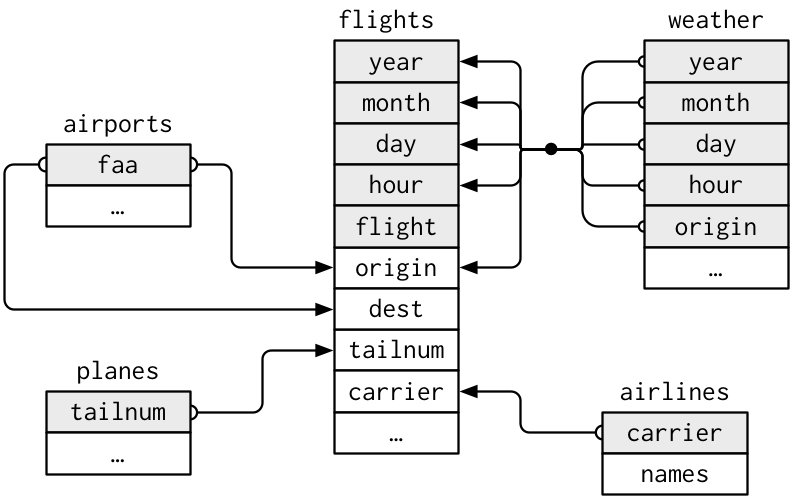
\includegraphics[width=0.5\textwidth,height=\textheight]{relational-nycflights.png}

Para nycflights13:

\begin{itemize}
\item
  \emph{flights} se conectam a \emph{planes} através de uma única
  variável, \emph{tailnum}.
\item
  \emph{flights} se conecta a \emph{airlines} pela vaariável
  \emph{carrier}
\item
  \emph{flights} se conecta a \emph{airports} de duas maneiras: pelas
  variáveis \emph{origin} e \emph{dest}
\item
  \emph{flights} se conecta a \emph{weather} através de \emph{origin} (o
  lugar), \emph{year}, \emph{month}, \emph{day} e \emph{hour}.
\end{itemize}

\hypertarget{exercuxedcios}{%
\paragraph{Exercícios}\label{exercuxedcios}}

1 - Imagine que você gostaria de traçar(aproximadamente)a rota que cada
avião faz de sua origem até seu destino. Quais variáveis você precisaria
usar? Quais variáveis você precisaria combinar?

2 - Me esqueci de desenhar a relação entre \emph{weather} e
\emph{airports}. Qual e a relação e como ela deveria aparecer no
diagrama mostrado anteriormente?

3 - \emph{weather} contêm apenas informações dos aeroportos de origem
(NYC). Se o dataframe também tivesse dados sobre todos os aeorportos dos
USA, que relação adicional esta tabela teria com \emph{flights}?

4 - Sabemos que alguns dias do ano são ``especiais'', que menos vôos
ocorrem nesses dias. Como você representaria estes dados em um data
frame? Quais seriam as chaves primárias desta tabela? Como ela se
conectaria com as tabela existentes?

\hypertarget{keys}{%
\paragraph{keys}\label{keys}}

As variáveis usadas para conectar cada par de tabelas são chamadas de
keys ou chaves. Uma chave é uma variável (ou conjunto de variáveis) que
identifica unicamente uma observação.

Existem dois tipos de chaves:

\begin{itemize}
\item
  Chave primária(primary key): identifica uma observação única em sua
  própria tabela. Por exemplo, \emph{planes\$tailnum} é uma chave
  primária porque identifica unicamente cada avião na tabela
  \emph{planes}.
\item
  Foreign Key: Identifica uma observação única em outra tabela. Por
  exemplo, \emph{flights\$tailnum} é uma Foreign Key porque apareça na
  tabela \emph{flights} onde relaciona cada vôo a a um avião único.
\end{itemize}

Uma variável também pode ser os dois tipos de chave ao mesmo tempo. Por
exemplo, \emph{origin} é parte da chave primária de \emph{weather} e
tambem é foreign key da tabela \emph{airport}.

Uma vez que você tenha identificado as chaves primárias em suas tabelas,
é boa prática verificar se elas realmente identificam unicamente cada
observação. Podemos fazer isso com \emph{count()}, contando as chaves
primárias e procurando por entradas onde \emph{n} é maior que um:

\begin{Shaded}
\begin{Highlighting}[]
\NormalTok{planes }\OperatorTok\StringTok{ }
\StringTok{  }\KeywordTok{count}\NormalTok{(tailnum) }\OperatorTok\StringTok{ }
\StringTok{  }\KeywordTok{filter}\NormalTok{(n }\OperatorTok{>}\StringTok{ }\DecValTok{1}\NormalTok{)}
\end{Highlighting}
\end{Shaded}

\begin{verbatim}
## # A tibble: 0 x 2
## # ... with 2 variables: tailnum <chr>, n <int>
\end{verbatim}

\begin{Shaded}
\begin{Highlighting}[]
\NormalTok{weather }\OperatorTok\StringTok{ }
\StringTok{  }\KeywordTok{count}\NormalTok{(year, month, day, hour, origin) }\OperatorTok\StringTok{ }
\StringTok{  }\KeywordTok{filter}\NormalTok{(n }\OperatorTok{>}\StringTok{ }\DecValTok{1}\NormalTok{)}
\end{Highlighting}
\end{Shaded}

\begin{verbatim}
## # A tibble: 3 x 6
##    year month   day  hour origin     n
##   <int> <int> <int> <int> <chr>  <int>
## 1  2013    11     3     1 EWR        2
## 2  2013    11     3     1 JFK        2
## 3  2013    11     3     1 LGA        2
\end{verbatim}

Pode acontecer de uma tabela não possuir uma chave primária explicita:
cada linha é uma observação, mas nenhuma combinação de variáveis a
identifica de forma confiável. Por exeplo, qual é a chave primária na
tabela \emph{flights}? Você pode pensar que seria a data mais o número
do vôo ou tail number(número da cauda), mas nenhuma das duas é única.

\begin{Shaded}
\begin{Highlighting}[]
\NormalTok{flights }\OperatorTok\StringTok{ }
\StringTok{  }\KeywordTok{count}\NormalTok{(year, month, day, flight) }\OperatorTok\StringTok{ }
\StringTok{  }\KeywordTok{filter}\NormalTok{(n }\OperatorTok{>}\StringTok{ }\DecValTok{1}\NormalTok{)}
\end{Highlighting}
\end{Shaded}

\begin{verbatim}
## # A tibble: 29,768 x 5
##     year month   day flight     n
##    <int> <int> <int>  <int> <int>
##  1  2013     1     1      1     2
##  2  2013     1     1      3     2
##  3  2013     1     1      4     2
##  4  2013     1     1     11     3
##  5  2013     1     1     15     2
##  6  2013     1     1     21     2
##  7  2013     1     1     27     4
##  8  2013     1     1     31     2
##  9  2013     1     1     32     2
## 10  2013     1     1     35     2
## # ... with 29,758 more rows
\end{verbatim}

\begin{Shaded}
\begin{Highlighting}[]
\NormalTok{flights }\OperatorTok\StringTok{ }
\StringTok{  }\KeywordTok{count}\NormalTok{(year, month, day, tailnum) }\OperatorTok\StringTok{ }
\StringTok{  }\KeywordTok{filter}\NormalTok{(n }\OperatorTok{>}\StringTok{ }\DecValTok{1}\NormalTok{)}
\end{Highlighting}
\end{Shaded}

\begin{verbatim}
## # A tibble: 64,928 x 5
##     year month   day tailnum     n
##    <int> <int> <int> <chr>   <int>
##  1  2013     1     1 N0EGMQ      2
##  2  2013     1     1 N11189      2
##  3  2013     1     1 N11536      2
##  4  2013     1     1 N11544      3
##  5  2013     1     1 N11551      2
##  6  2013     1     1 N12540      2
##  7  2013     1     1 N12567      2
##  8  2013     1     1 N13123      2
##  9  2013     1     1 N13538      3
## 10  2013     1     1 N13566      3
## # ... with 64,918 more rows
\end{verbatim}

Se uma tabela não possui uma chave primária, pode ser bom criar uma com
as funções \emph{mutate()} e \emph{row\_number()}. Assim fica mais fácil
relacionar observações se os dados foram filtrados é você quer verificar
novamente os dados originais. Este tipo de chave é chamada de
\emph{surrogate key}.

Uma chave primária e sua correspondente foreign key em outra tabela
formam uma realação. Relações são geralmente de um para muitos. Por
exemplo,

\hypertarget{exercuxedcios-1}{%
\paragraph{Exercícios}\label{exercuxedcios-1}}

1 - Faça uma chave surrogate para a tabela \emph{flights}

2 - Identifique as chaves nos seguintes conjuntos de dados:

\begin{enumerate}
\def\labelenumi{\arabic{enumi}.}
\tightlist
\item
  Lahman::Batting,
\item
  babynames::babynames
\item
  nasaweather::atmos
\item
  fueleconomy::vehicles
\item
  ggplot2::diamonds
\end{enumerate}

(talvez seja necessário instalar alguns pacotes e ler a documentação)

3 - Faça um diagrama ilustrando as conexões entre as tabelas
\emph{Batting}, \emph{Master}, e \emph{Salaries} no pacote Lahman. Faça
outro diagrama que deve mostrar as relações entre \emph{Master},
\emph{Managers}, \emph{AwardsManagers}.

Como você caracterizaria a relação entre as tabelas \emph{Batting},
\emph{Pitching} e \emph{Fielding}.

\hypertarget{mutating-joins}{%
\paragraph{Mutating joins}\label{mutating-joins}}

Como o \emph{mutate()}, as funções join adicionam variáveis a direita,
então, se houverem muitas variáveis na tabela elas não aparecerão
printadas, por este motivo iremos estreitar as tabelas dos próximos
exemplos, criando tabelas menos largas(com menos colunas)

\begin{Shaded}
\begin{Highlighting}[]
\NormalTok{flights2 <-}\StringTok{ }\NormalTok{flights }\OperatorTok\StringTok{ }
\StringTok{  }\KeywordTok{select}\NormalTok{(year}\OperatorTok{:}\NormalTok{day, hour, origin, dest, tailnum, carrier)}
\NormalTok{flights2}
\end{Highlighting}
\end{Shaded}

\begin{verbatim}
## # A tibble: 336,776 x 8
##     year month   day  hour origin dest  tailnum carrier
##    <int> <int> <int> <dbl> <chr>  <chr> <chr>   <chr>  
##  1  2013     1     1     5 EWR    IAH   N14228  UA     
##  2  2013     1     1     5 LGA    IAH   N24211  UA     
##  3  2013     1     1     5 JFK    MIA   N619AA  AA     
##  4  2013     1     1     5 JFK    BQN   N804JB  B6     
##  5  2013     1     1     6 LGA    ATL   N668DN  DL     
##  6  2013     1     1     5 EWR    ORD   N39463  UA     
##  7  2013     1     1     6 EWR    FLL   N516JB  B6     
##  8  2013     1     1     6 LGA    IAD   N829AS  EV     
##  9  2013     1     1     6 JFK    MCO   N593JB  B6     
## 10  2013     1     1     6 LGA    ORD   N3ALAA  AA     
## # ... with 336,766 more rows
\end{verbatim}

(Lembre-se, no RStudio é possível usar \_view() para evitar este tipo de
problema.)

Imagine que você queira adicionar os nomes de linhas aéreas à tabela
\emph{flights2}. Você pode combinar as tabelas \emph{flights} e
\emph{Flights2} com um \emph{left\_join()}:

\begin{Shaded}
\begin{Highlighting}[]
\NormalTok{flights2 }\OperatorTok
\StringTok{  }\KeywordTok{select}\NormalTok{(}\OperatorTok{-}\NormalTok{origin, }\OperatorTok{-}\NormalTok{dest) }\OperatorTok\StringTok{ }
\StringTok{  }\KeywordTok{left_join}\NormalTok{(airlines, }\DataTypeTok{by =} \StringTok{"carrier"}\NormalTok{)}
\end{Highlighting}
\end{Shaded}

\begin{verbatim}
## # A tibble: 336,776 x 7
##     year month   day  hour tailnum carrier name                    
##    <int> <int> <int> <dbl> <chr>   <chr>   <chr>                   
##  1  2013     1     1     5 N14228  UA      United Air Lines Inc.   
##  2  2013     1     1     5 N24211  UA      United Air Lines Inc.   
##  3  2013     1     1     5 N619AA  AA      American Airlines Inc.  
##  4  2013     1     1     5 N804JB  B6      JetBlue Airways         
##  5  2013     1     1     6 N668DN  DL      Delta Air Lines Inc.    
##  6  2013     1     1     5 N39463  UA      United Air Lines Inc.   
##  7  2013     1     1     6 N516JB  B6      JetBlue Airways         
##  8  2013     1     1     6 N829AS  EV      ExpressJet Airlines Inc.
##  9  2013     1     1     6 N593JB  B6      JetBlue Airways         
## 10  2013     1     1     6 N3ALAA  AA      American Airlines Inc.  
## # ... with 336,766 more rows
\end{verbatim}

Como resultado desta junção temos uma nova variável, \emph{name}. Por
este motivo chamamos este tipo de join de mutating join. Neste caso,
seria possível ter o mesmo resultado usando a função \emph{mutate()}.

\begin{Shaded}
\begin{Highlighting}[]
\NormalTok{flights2 }\OperatorTok
\StringTok{  }\KeywordTok{select}\NormalTok{(}\OperatorTok{-}\NormalTok{origin, }\OperatorTok{-}\NormalTok{dest) }\OperatorTok\StringTok{ }
\StringTok{  }\KeywordTok{mutate}\NormalTok{(}\DataTypeTok{name =}\NormalTok{ airlines}\OperatorTok{$}\NormalTok{name[}\KeywordTok{match}\NormalTok{(carrier, airlines}\OperatorTok{$}\NormalTok{carrier)])}
\end{Highlighting}
\end{Shaded}

\begin{verbatim}
## # A tibble: 336,776 x 7
##     year month   day  hour tailnum carrier name                    
##    <int> <int> <int> <dbl> <chr>   <chr>   <chr>                   
##  1  2013     1     1     5 N14228  UA      United Air Lines Inc.   
##  2  2013     1     1     5 N24211  UA      United Air Lines Inc.   
##  3  2013     1     1     5 N619AA  AA      American Airlines Inc.  
##  4  2013     1     1     5 N804JB  B6      JetBlue Airways         
##  5  2013     1     1     6 N668DN  DL      Delta Air Lines Inc.    
##  6  2013     1     1     5 N39463  UA      United Air Lines Inc.   
##  7  2013     1     1     6 N516JB  B6      JetBlue Airways         
##  8  2013     1     1     6 N829AS  EV      ExpressJet Airlines Inc.
##  9  2013     1     1     6 N593JB  B6      JetBlue Airways         
## 10  2013     1     1     6 N3ALAA  AA      American Airlines Inc.  
## # ... with 336,766 more rows
\end{verbatim}

Entretanto, este método não é prático quando se precisa relacionar
muitas variáveis, além de necessitar de uma leitura mais minunciosa para
o seu entendimento.

\hypertarget{entendendo-joins}{%
\paragraph{Entendendo Joins}\label{entendendo-joins}}

Será mais fácil entender como funcionam os joins com uma representação
visual de seu funcionamento:

\begin{figure}
\centering
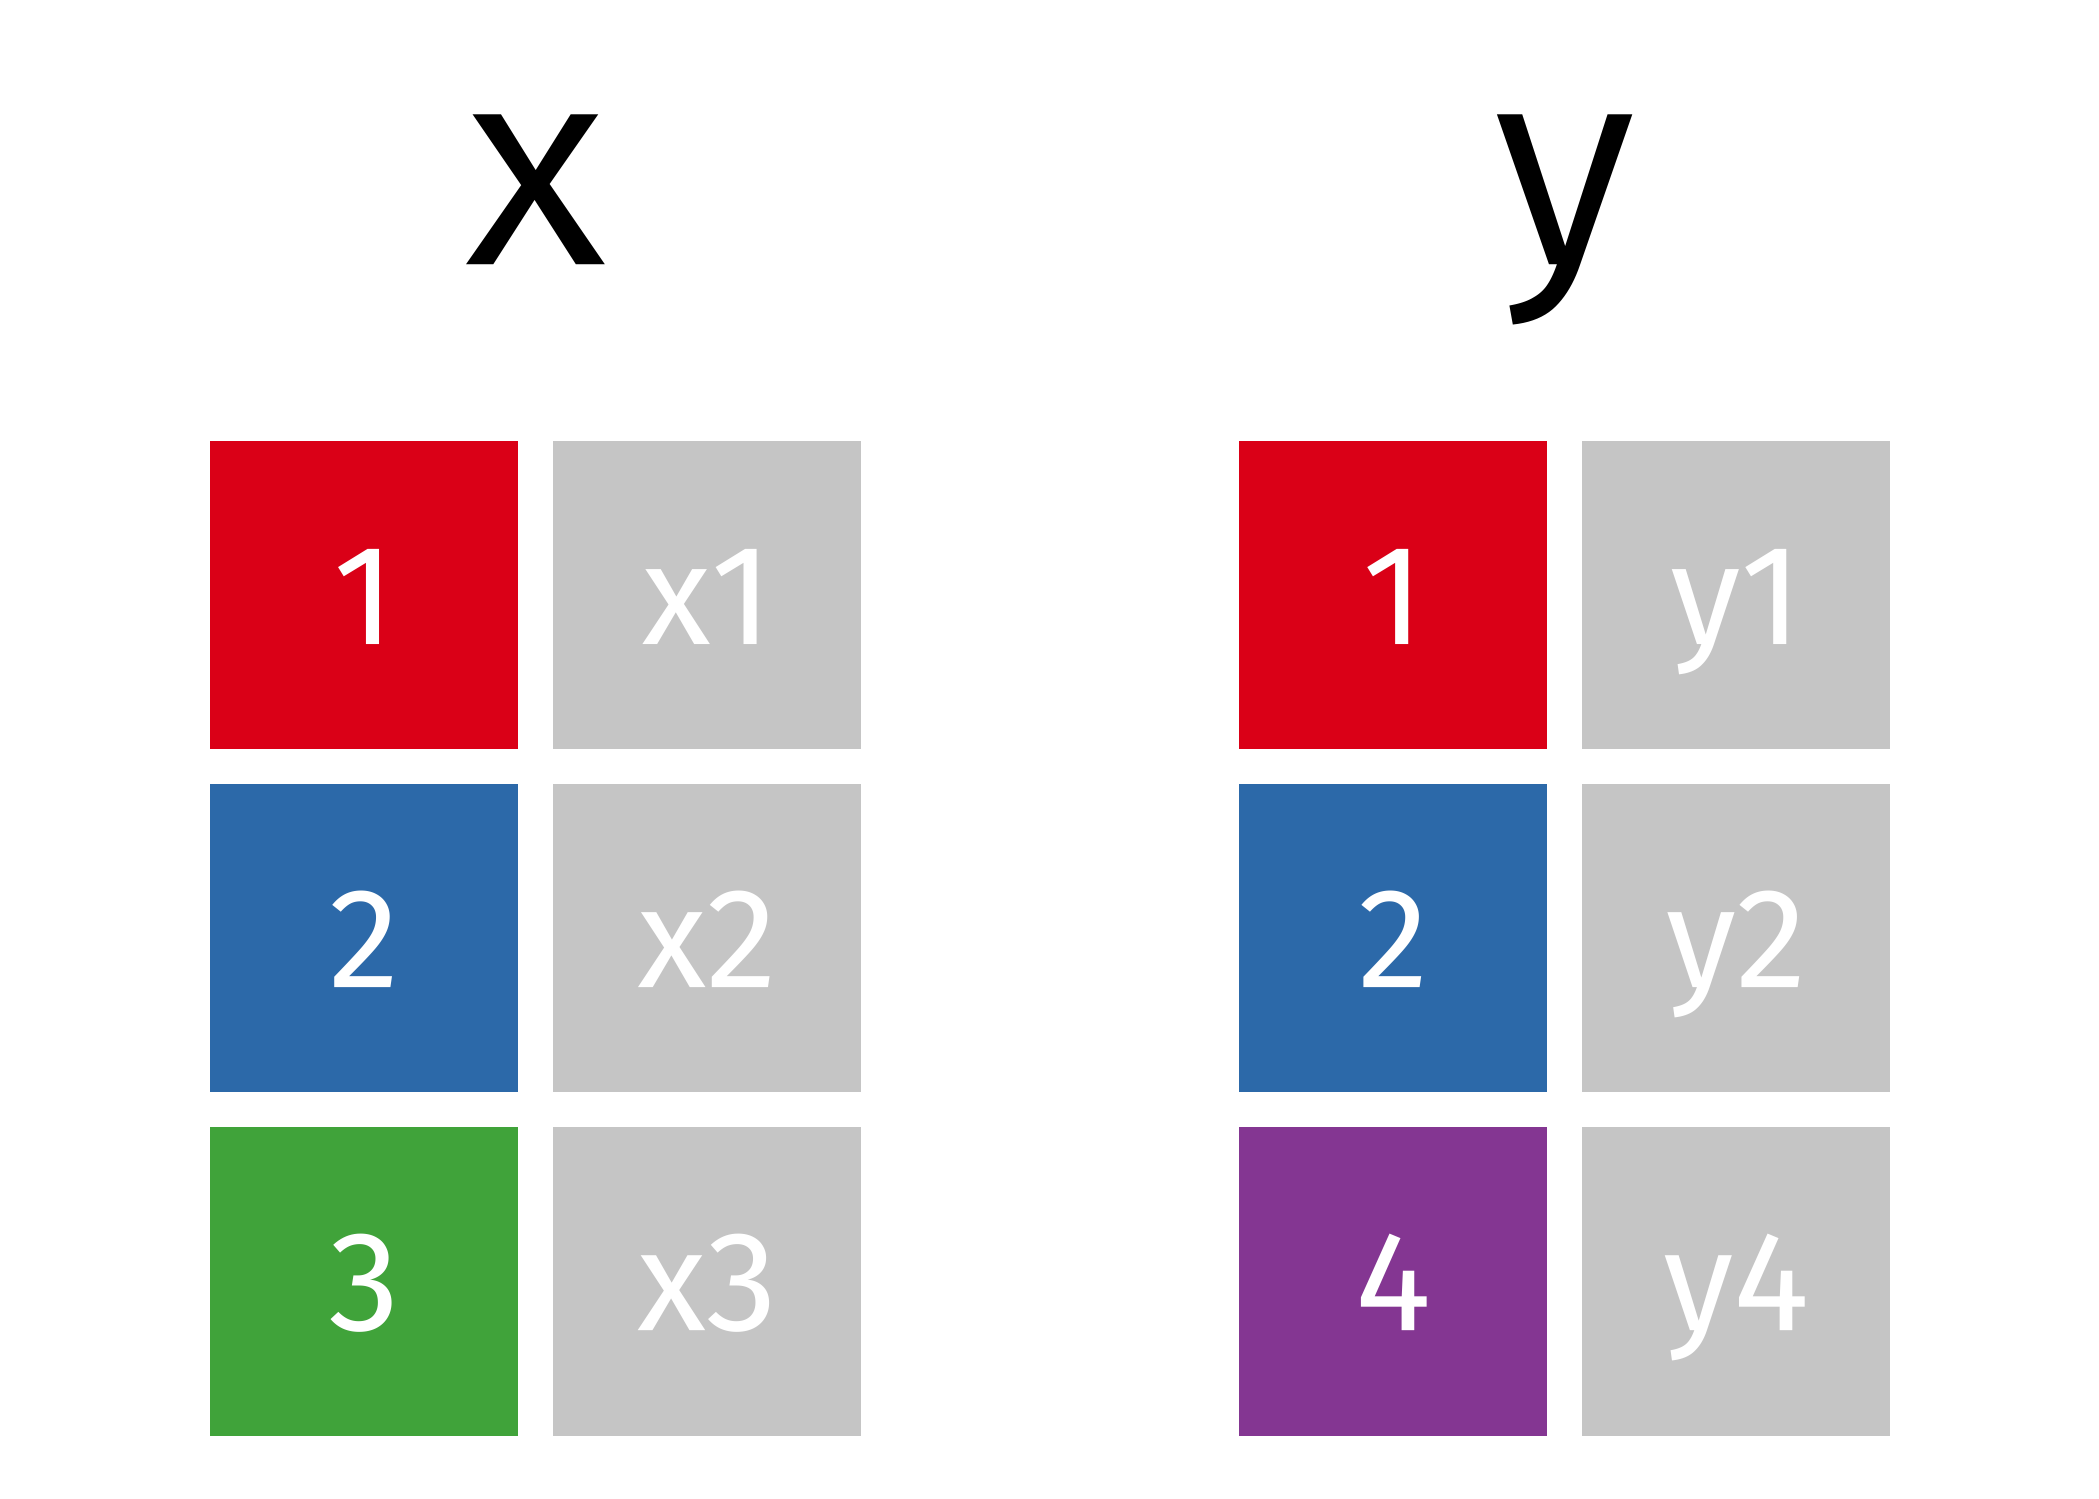
\includegraphics[width=0.5\textwidth,height=\textheight]{original-dfs.png}
\caption{\emph{Fonte:
\url{https://www.garrickadenbuie.com/project/tidyexplain/}}}
\end{figure}

\begin{Shaded}
\begin{Highlighting}[]
\CommentTok{#x}
\CommentTok{#> # A tibble: 3 x 2}
\CommentTok{#>      id x    }
\CommentTok{#>   <int> <chr>}
\CommentTok{#> 1     1 x1   }
\CommentTok{#> 2     2 x2   }
\CommentTok{#> 3     3 x3}
\CommentTok{#y}
\CommentTok{#> # A tibble: 3 x 2}
\CommentTok{#>      id y    }
\CommentTok{#>   <int> <chr>}
\CommentTok{#> 1     1 y1   }
\CommentTok{#> 2     2 y2   }
\CommentTok{#> 3     4 y4}
\end{Highlighting}
\end{Shaded}

As colunas coloridas representam a variável ``chave'': usadas para
relacionas as linhas(observações) entre as duas tabelas. A coluna cinza
representa os valores.

Um join é uma maneira de conectar cada linha em x a zero, uma ou mais
linhas em Y. Será possível entender melhor este funcionamento nas
tabelas animadas que serão mostradas nos próximos exemplos.

\hypertarget{inner-join}{%
\paragraph{Inner Join}\label{inner-join}}

É o tipo mais simples de Join, relaciona pares de observações quando
suas chaves são iguais.

\begin{figure}
\centering
\includegraphics[width=0.5\textwidth,height=\textheight]{inner-join.gif}
\caption{\emph{Fonte:
\url{https://www.garrickadenbuie.com/project/tidyexplain/}}}
\end{figure}

\begin{Shaded}
\begin{Highlighting}[]
\CommentTok{#inner_join(x, y, by = "id")}
\CommentTok{#> # A tibble: 2 x 3}
\CommentTok{#>      id x     y    }
\CommentTok{#>   <int> <chr> <chr>}
\CommentTok{#> 1     1 x1    y1   }
\CommentTok{#> 2     2 x2    y2}
\end{Highlighting}
\end{Shaded}

As observações não relacionadas são ignoradas no output. Não se costuma
usar este tipo de join em análises pois facilita a perda de observações.

\hypertarget{outer-joins}{%
\paragraph{Outer Joins}\label{outer-joins}}

Preserva observações que aparecem em pelo menos uma das tabelas, existem
três tipos:

\begin{itemize}
\tightlist
\item
  Left join, mantem as observações de X.
\end{itemize}

\begin{figure}
\centering
\includegraphics[width=0.5\textwidth,height=\textheight]{left-join.gif}
\caption{\emph{Fonte:
\url{https://www.garrickadenbuie.com/project/tidyexplain/}}}
\end{figure}

\begin{itemize}
\tightlist
\item
  right join, mantem as observações em y.
\end{itemize}

\begin{figure}
\centering
\includegraphics[width=0.5\textwidth,height=\textheight]{right-join.gif}
\caption{\emph{Fonte:
\url{https://www.garrickadenbuie.com/project/tidyexplain/}}}
\end{figure}

\begin{itemize}
\tightlist
\item
  Full join, mantem as observações tanto em x quanto em y.
\end{itemize}

\begin{figure}
\centering
\includegraphics[width=0.5\textwidth,height=\textheight]{full-join.gif}
\caption{\emph{Fonte:
\url{https://www.garrickadenbuie.com/project/tidyexplain/}}}
\end{figure}

O join mais usado é o left join, você pode trazer dados de outra tabela
preservando as observações originais.

Outra maneira de representar os joins é através de um diagrama de Venn:

\begin{itemize}
\tightlist
\item
  Full join, mantem as observações tanto em x quanto em y.
\end{itemize}

\begin{figure}
\centering
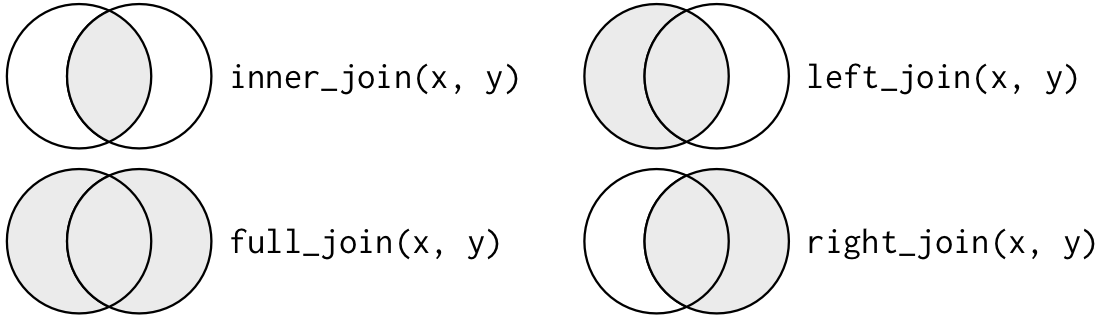
\includegraphics[width=0.5\textwidth,height=\textheight]{join-venn.png}
\caption{\emph{Fonte: Hickham e Grolemund - Relational data}}
\end{figure}

\hypertarget{chaves-duplicadas}{%
\paragraph{Chaves duplicadas}\label{chaves-duplicadas}}

Até agora, em todos os diagramas assumimos que as chaves eram únicas,
porém, não é sempre o caso. Agora vamos entender o que acontece quando
as chaves não são únicas. Existem duas possibilidades:

1 - Uma das tabelas tem chaves duplicadas. isso acontece quando se quer
adicionar informações adicionais, assim cria-se uma relação de um para
muitos.

\begin{figure}
\centering
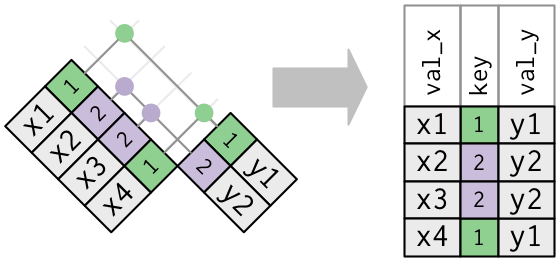
\includegraphics[width=0.5\textwidth,height=\textheight]{join-one-to-many.png}
\caption{\emph{Fonte: Hickham e Grolemund - Relational data}}
\end{figure}

\begin{Shaded}
\begin{Highlighting}[]
\NormalTok{x <-}\StringTok{ }\KeywordTok{tribble}\NormalTok{(}
  \OperatorTok{~}\NormalTok{key, }\OperatorTok{~}\NormalTok{val_x,}
     \DecValTok{1}\NormalTok{, }\StringTok{"x1"}\NormalTok{,}
     \DecValTok{2}\NormalTok{, }\StringTok{"x2"}\NormalTok{,}
     \DecValTok{2}\NormalTok{, }\StringTok{"x3"}\NormalTok{,}
     \DecValTok{1}\NormalTok{, }\StringTok{"x4"}
\NormalTok{)}
\NormalTok{y <-}\StringTok{ }\KeywordTok{tribble}\NormalTok{(}
  \OperatorTok{~}\NormalTok{key, }\OperatorTok{~}\NormalTok{val_y,}
     \DecValTok{1}\NormalTok{, }\StringTok{"y1"}\NormalTok{,}
     \DecValTok{2}\NormalTok{, }\StringTok{"y2"}
\NormalTok{)}
\KeywordTok{left_join}\NormalTok{(x, y, }\DataTypeTok{by =} \StringTok{"key"}\NormalTok{)}
\end{Highlighting}
\end{Shaded}

\begin{verbatim}
## # A tibble: 4 x 3
##     key val_x val_y
##   <dbl> <chr> <chr>
## 1     1 x1    y1   
## 2     2 x2    y2   
## 3     2 x3    y2   
## 4     1 x4    y1
\end{verbatim}

2 - Existem chaves duplicadas nas duas tabelas. Isto geralmente é um
erro porque em nenhuma das duas tabelas as chaves identificam de forma
única uma observação.

\begin{figure}
\centering
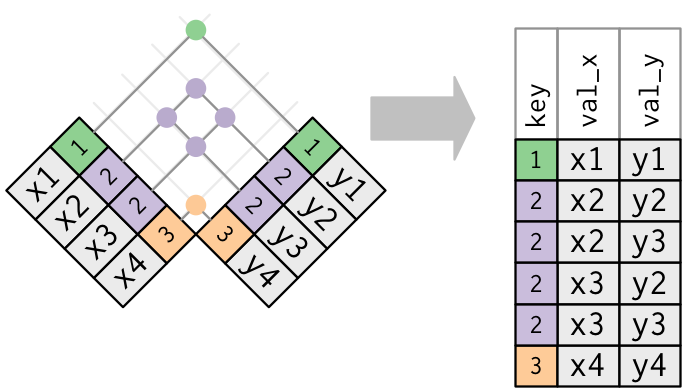
\includegraphics[width=0.5\textwidth,height=\textheight]{join-many-to-many.png}
\caption{\emph{Fonte: Hickham e Grolemund - Relational data}}
\end{figure}

\begin{Shaded}
\begin{Highlighting}[]
\NormalTok{x <-}\StringTok{ }\KeywordTok{tribble}\NormalTok{(}
  \OperatorTok{~}\NormalTok{key, }\OperatorTok{~}\NormalTok{val_x,}
     \DecValTok{1}\NormalTok{, }\StringTok{"x1"}\NormalTok{,}
     \DecValTok{2}\NormalTok{, }\StringTok{"x2"}\NormalTok{,}
     \DecValTok{2}\NormalTok{, }\StringTok{"x3"}\NormalTok{,}
     \DecValTok{3}\NormalTok{, }\StringTok{"x4"}
\NormalTok{)}
\NormalTok{y <-}\StringTok{ }\KeywordTok{tribble}\NormalTok{(}
  \OperatorTok{~}\NormalTok{key, }\OperatorTok{~}\NormalTok{val_y,}
     \DecValTok{1}\NormalTok{, }\StringTok{"y1"}\NormalTok{,}
     \DecValTok{2}\NormalTok{, }\StringTok{"y2"}\NormalTok{,}
     \DecValTok{2}\NormalTok{, }\StringTok{"y3"}\NormalTok{,}
     \DecValTok{3}\NormalTok{, }\StringTok{"y4"}
\NormalTok{)}
\KeywordTok{left_join}\NormalTok{(x, y, }\DataTypeTok{by =} \StringTok{"key"}\NormalTok{)}
\end{Highlighting}
\end{Shaded}

\begin{verbatim}
## # A tibble: 6 x 3
##     key val_x val_y
##   <dbl> <chr> <chr>
## 1     1 x1    y1   
## 2     2 x2    y2   
## 3     2 x2    y3   
## 4     2 x3    y2   
## 5     2 x3    y3   
## 6     3 x4    y4
\end{verbatim}

\hypertarget{definindo-as-colunas-chave}{%
\paragraph{Definindo as colunas
chave}\label{definindo-as-colunas-chave}}

Até agora, os pares de tabelas foram sempre unidas por uma única
variável e essa variável tem o mesmo nome nas duas tambelas. Esta
restrição foi codificada por \emph{by=``key''} . É possível usar outros
valores para \emph{by} para conectar tabelas de outras maneiras:

\begin{itemize}
\tightlist
\item
  O deafault, \emph{by=null}, usa todas as variáveis que aparecem nas
  duas tabelas, chamado de união natural. Por exemplo, as tabelas
  flights e weather se relacionam em suas variáveis comuns: year, month,
  day, hour e origin.
\end{itemize}

\begin{Shaded}
\begin{Highlighting}[]
\NormalTok{flights2 }\OperatorTok\StringTok{ }
\StringTok{  }\KeywordTok{left_join}\NormalTok{(weather)}
\end{Highlighting}
\end{Shaded}

\begin{verbatim}
## Joining, by = c("year", "month", "day", "hour", "origin")
\end{verbatim}

\begin{verbatim}
## # A tibble: 336,776 x 18
##     year month   day  hour origin dest  tailnum carrier  temp  dewp humid
##    <int> <int> <int> <dbl> <chr>  <chr> <chr>   <chr>   <dbl> <dbl> <dbl>
##  1  2013     1     1     5 EWR    IAH   N14228  UA       39.0  28.0  64.4
##  2  2013     1     1     5 LGA    IAH   N24211  UA       39.9  25.0  54.8
##  3  2013     1     1     5 JFK    MIA   N619AA  AA       39.0  27.0  61.6
##  4  2013     1     1     5 JFK    BQN   N804JB  B6       39.0  27.0  61.6
##  5  2013     1     1     6 LGA    ATL   N668DN  DL       39.9  25.0  54.8
##  6  2013     1     1     5 EWR    ORD   N39463  UA       39.0  28.0  64.4
##  7  2013     1     1     6 EWR    FLL   N516JB  B6       37.9  28.0  67.2
##  8  2013     1     1     6 LGA    IAD   N829AS  EV       39.9  25.0  54.8
##  9  2013     1     1     6 JFK    MCO   N593JB  B6       37.9  27.0  64.3
## 10  2013     1     1     6 LGA    ORD   N3ALAA  AA       39.9  25.0  54.8
## # ... with 336,766 more rows, and 7 more variables: wind_dir <dbl>,
## #   wind_speed <dbl>, wind_gust <dbl>, precip <dbl>, pressure <dbl>,
## #   visib <dbl>, time_hour <dttm>
\end{verbatim}

\begin{itemize}
\tightlist
\item
  Um vetor caracter, \emph{by=``x''}. É como um join natural, mas usa
  apenas algumas das variáveis comuns. Por exemplo, flights e planes tem
  variáveis \emph{year}, mas elas tem significados diferentes então
  unimos as tabelas apenas por \emph{tailnum}
\end{itemize}

\begin{Shaded}
\begin{Highlighting}[]
\NormalTok{flights2 }\OperatorTok\StringTok{ }
\StringTok{  }\KeywordTok{left_join}\NormalTok{(planes, }\DataTypeTok{by =} \StringTok{"tailnum"}\NormalTok{)}
\end{Highlighting}
\end{Shaded}

\begin{verbatim}
## # A tibble: 336,776 x 16
##    year.x month   day  hour origin dest  tailnum carrier year.y type 
##     <int> <int> <int> <dbl> <chr>  <chr> <chr>   <chr>    <int> <chr>
##  1   2013     1     1     5 EWR    IAH   N14228  UA        1999 Fixe~
##  2   2013     1     1     5 LGA    IAH   N24211  UA        1998 Fixe~
##  3   2013     1     1     5 JFK    MIA   N619AA  AA        1990 Fixe~
##  4   2013     1     1     5 JFK    BQN   N804JB  B6        2012 Fixe~
##  5   2013     1     1     6 LGA    ATL   N668DN  DL        1991 Fixe~
##  6   2013     1     1     5 EWR    ORD   N39463  UA        2012 Fixe~
##  7   2013     1     1     6 EWR    FLL   N516JB  B6        2000 Fixe~
##  8   2013     1     1     6 LGA    IAD   N829AS  EV        1998 Fixe~
##  9   2013     1     1     6 JFK    MCO   N593JB  B6        2004 Fixe~
## 10   2013     1     1     6 LGA    ORD   N3ALAA  AA          NA <NA> 
## # ... with 336,766 more rows, and 6 more variables: manufacturer <chr>,
## #   model <chr>, engines <int>, seats <int>, speed <int>, engine <chr>
\end{verbatim}

\begin{itemize}
\tightlist
\item
  Um vetor caracter nomeado: \emph{by = c(``a'' = ``b'')} . Isso vai
  relacionar a variável a na tabela x a uma variável b na tabela y.
\end{itemize}

Por exemplo, se quisermos desenhar um mapa precisamos combinar os dados
de flights e airports que contem a localização de cada aeroporto. Cada
vôo tem uma origem e um destino \emph{airport}, então precisamos
especificar qual queremos unir a qual.

\begin{Shaded}
\begin{Highlighting}[]
\NormalTok{flights2 }\OperatorTok\StringTok{ }
\StringTok{  }\KeywordTok{left_join}\NormalTok{(airports, }\KeywordTok{c}\NormalTok{(}\StringTok{"dest"}\NormalTok{ =}\StringTok{ "faa"}\NormalTok{))}
\end{Highlighting}
\end{Shaded}

\begin{verbatim}
## # A tibble: 336,776 x 15
##     year month   day  hour origin dest  tailnum carrier name    lat   lon   alt
##    <int> <int> <int> <dbl> <chr>  <chr> <chr>   <chr>   <chr> <dbl> <dbl> <dbl>
##  1  2013     1     1     5 EWR    IAH   N14228  UA      Geor~  30.0 -95.3    97
##  2  2013     1     1     5 LGA    IAH   N24211  UA      Geor~  30.0 -95.3    97
##  3  2013     1     1     5 JFK    MIA   N619AA  AA      Miam~  25.8 -80.3     8
##  4  2013     1     1     5 JFK    BQN   N804JB  B6      <NA>   NA    NA      NA
##  5  2013     1     1     6 LGA    ATL   N668DN  DL      Hart~  33.6 -84.4  1026
##  6  2013     1     1     5 EWR    ORD   N39463  UA      Chic~  42.0 -87.9   668
##  7  2013     1     1     6 EWR    FLL   N516JB  B6      Fort~  26.1 -80.2     9
##  8  2013     1     1     6 LGA    IAD   N829AS  EV      Wash~  38.9 -77.5   313
##  9  2013     1     1     6 JFK    MCO   N593JB  B6      Orla~  28.4 -81.3    96
## 10  2013     1     1     6 LGA    ORD   N3ALAA  AA      Chic~  42.0 -87.9   668
## # ... with 336,766 more rows, and 3 more variables: tz <dbl>, dst <chr>,
## #   tzone <chr>
\end{verbatim}

\begin{Shaded}
\begin{Highlighting}[]
\NormalTok{flights2 }\OperatorTok\StringTok{ }
\StringTok{  }\KeywordTok{left_join}\NormalTok{(airports, }\KeywordTok{c}\NormalTok{(}\StringTok{"origin"}\NormalTok{ =}\StringTok{ "faa"}\NormalTok{))}
\end{Highlighting}
\end{Shaded}

\begin{verbatim}
## # A tibble: 336,776 x 15
##     year month   day  hour origin dest  tailnum carrier name    lat   lon   alt
##    <int> <int> <int> <dbl> <chr>  <chr> <chr>   <chr>   <chr> <dbl> <dbl> <dbl>
##  1  2013     1     1     5 EWR    IAH   N14228  UA      Newa~  40.7 -74.2    18
##  2  2013     1     1     5 LGA    IAH   N24211  UA      La G~  40.8 -73.9    22
##  3  2013     1     1     5 JFK    MIA   N619AA  AA      John~  40.6 -73.8    13
##  4  2013     1     1     5 JFK    BQN   N804JB  B6      John~  40.6 -73.8    13
##  5  2013     1     1     6 LGA    ATL   N668DN  DL      La G~  40.8 -73.9    22
##  6  2013     1     1     5 EWR    ORD   N39463  UA      Newa~  40.7 -74.2    18
##  7  2013     1     1     6 EWR    FLL   N516JB  B6      Newa~  40.7 -74.2    18
##  8  2013     1     1     6 LGA    IAD   N829AS  EV      La G~  40.8 -73.9    22
##  9  2013     1     1     6 JFK    MCO   N593JB  B6      John~  40.6 -73.8    13
## 10  2013     1     1     6 LGA    ORD   N3ALAA  AA      La G~  40.8 -73.9    22
## # ... with 336,766 more rows, and 3 more variables: tz <dbl>, dst <chr>,
## #   tzone <chr>
\end{verbatim}

\hypertarget{exercuxedcios-2}{%
\paragraph{Exercícios}\label{exercuxedcios-2}}

1 - Compute o atraso médio por destino, então una aos dados da tabela
\emph{airports}, assim você poderá mostrar a distribuição espacial dos
atrasos. Aqui esta um modo fácil de plotar um mapa dos estados unidos.

\begin{Shaded}
\begin{Highlighting}[]
\NormalTok{airports }\OperatorTok
\StringTok{  }\KeywordTok{semi_join}\NormalTok{(flights, }\KeywordTok{c}\NormalTok{(}\StringTok{"faa"}\NormalTok{ =}\StringTok{ "dest"}\NormalTok{)) }\OperatorTok
\StringTok{  }\KeywordTok{ggplot}\NormalTok{(}\KeywordTok{aes}\NormalTok{(lon, lat)) }\OperatorTok{+}
\StringTok{    }\KeywordTok{borders}\NormalTok{(}\StringTok{"state"}\NormalTok{) }\OperatorTok{+}
\StringTok{    }\KeywordTok{geom_point}\NormalTok{() }\OperatorTok{+}
\StringTok{    }\KeywordTok{coord_quickmap}\NormalTok{()}
\end{Highlighting}
\end{Shaded}

\includegraphics{reldata_files/figure-latex/unnamed-chunk-18-1.pdf}

Voce talvez queira usar \emph{size} ou \emph{color} dos pontos para
mostrar o atraso médio em cada aeroporto.

2 - Adicione a localização da origem e do destino a tabela
\emph{flights}

3 - Existe relação entre a idade do avião e seus atrasos?

4 - Que condições climáticas influenciam nos atrasos?

5 -O que aconteceu em 13 de junho de 2013? Mostre o padrão espacial de
atrasos, use o google para fazer uma referência crusada com o clima no
dia.

\hypertarget{filtering-joins}{%
\paragraph{Filtering Joins}\label{filtering-joins}}

Filtering joins relacionam observações do mesmo modo que muatating
joins, mas afetam as observações, não as variáveis. Existem 2 tipos.

\begin{itemize}
\tightlist
\item
  \emph{semi\_join(x,y)} mantêm todas as orbservações em x que tenham
  uma correspondência em y.
\end{itemize}

\begin{Shaded}
\begin{Highlighting}[]
\CommentTok{#semi_join(x, y, by = "id")}
\CommentTok{#> # A tibble: 2 x 2}
\CommentTok{#>      id x    }
\CommentTok{#>   <int> <chr>}
\CommentTok{#> 1     1 x1   }
\CommentTok{#> 2     2 x2}
\end{Highlighting}
\end{Shaded}

\begin{figure}
\centering
\includegraphics[width=0.5\textwidth,height=\textheight]{semi-join.gif}
\caption{\emph{Fonte:
\url{https://www.garrickadenbuie.com/project/tidyexplain/}}}
\end{figure}

\begin{itemize}
\tightlist
\item
  \emph{anti\_join(x,y)} Ignora todas as observações em x que tenham
  correspondência em y.
\end{itemize}

\begin{Shaded}
\begin{Highlighting}[]
\CommentTok{#anti_join(x, y, by = "id")}
\CommentTok{#> # A tibble: 1 x 2}
\CommentTok{#>      id x    }
\CommentTok{#>   <int> <chr>}
\CommentTok{#> 1     3 x3}
\end{Highlighting}
\end{Shaded}

\begin{figure}
\centering
\includegraphics[width=0.5\textwidth,height=\textheight]{anti-join.gif}
\caption{\emph{Fonte:
\url{https://www.garrickadenbuie.com/project/tidyexplain/}}}
\end{figure}

Semi-joins são úteis ao relacionar tabelas de sumário filtradas de volta
para as linhas originais. Por exemplo, imagine que você encontrou os 10
destinos mais populares:

\begin{Shaded}
\begin{Highlighting}[]
\NormalTok{top_dest <-}\StringTok{ }\NormalTok{flights }\OperatorTok
\StringTok{  }\KeywordTok{count}\NormalTok{(dest, }\DataTypeTok{sort =} \OtherTok{TRUE}\NormalTok{) }\OperatorTok
\StringTok{  }\KeywordTok{head}\NormalTok{(}\DecValTok{10}\NormalTok{)}
\NormalTok{top_dest}
\end{Highlighting}
\end{Shaded}

\begin{verbatim}
## # A tibble: 10 x 2
##    dest      n
##    <chr> <int>
##  1 ORD   17283
##  2 ATL   17215
##  3 LAX   16174
##  4 BOS   15508
##  5 MCO   14082
##  6 CLT   14064
##  7 SFO   13331
##  8 FLL   12055
##  9 MIA   11728
## 10 DCA    9705
\end{verbatim}

Agora você quer encontrar cada vôo que foi para cada um destes destinos.
Você poderia fazer um filtro:

\begin{Shaded}
\begin{Highlighting}[]
\NormalTok{flights }\OperatorTok\StringTok{ }
\StringTok{  }\KeywordTok{filter}\NormalTok{(dest }\OperatorTok\StringTok{ }\NormalTok{top_dest}\OperatorTok{$}\NormalTok{dest)}
\end{Highlighting}
\end{Shaded}

\begin{verbatim}
## # A tibble: 141,145 x 19
##     year month   day dep_time sched_dep_time dep_delay arr_time sched_arr_time
##    <int> <int> <int>    <int>          <int>     <dbl>    <int>          <int>
##  1  2013     1     1      542            540         2      923            850
##  2  2013     1     1      554            600        -6      812            837
##  3  2013     1     1      554            558        -4      740            728
##  4  2013     1     1      555            600        -5      913            854
##  5  2013     1     1      557            600        -3      838            846
##  6  2013     1     1      558            600        -2      753            745
##  7  2013     1     1      558            600        -2      924            917
##  8  2013     1     1      558            600        -2      923            937
##  9  2013     1     1      559            559         0      702            706
## 10  2013     1     1      600            600         0      851            858
## # ... with 141,135 more rows, and 11 more variables: arr_delay <dbl>,
## #   carrier <chr>, flight <int>, tailnum <chr>, origin <chr>, dest <chr>,
## #   air_time <dbl>, distance <dbl>, hour <dbl>, minute <dbl>, time_hour <dttm>
\end{verbatim}

Mas é difícil fazer o mesmo para múltiplas variáveis. Por exemplo,
imagine que você encontrou os 10 dias com maiores atrasos médios. Como
você construiria um filtro que usasse \emph{year}, \emph{month} e
\emph{day} para relacionar a de volta a tabela \emph{flights}?

Ao invés disso você pode usar um semi-join, que conecta as duas tabelas
como um mutating join, mas ao invés de adicionar novas colunas, mantem
apenas as colunas de x que tem uma correspondência em y.

\emph{y}

\begin{Shaded}
\begin{Highlighting}[]
\NormalTok{flights }\OperatorTok\StringTok{ }
\StringTok{  }\KeywordTok{semi_join}\NormalTok{(top_dest)}
\end{Highlighting}
\end{Shaded}

\begin{verbatim}
## Joining, by = "dest"
\end{verbatim}

\begin{verbatim}
## # A tibble: 141,145 x 19
##     year month   day dep_time sched_dep_time dep_delay arr_time sched_arr_time
##    <int> <int> <int>    <int>          <int>     <dbl>    <int>          <int>
##  1  2013     1     1      542            540         2      923            850
##  2  2013     1     1      554            600        -6      812            837
##  3  2013     1     1      554            558        -4      740            728
##  4  2013     1     1      555            600        -5      913            854
##  5  2013     1     1      557            600        -3      838            846
##  6  2013     1     1      558            600        -2      753            745
##  7  2013     1     1      558            600        -2      924            917
##  8  2013     1     1      558            600        -2      923            937
##  9  2013     1     1      559            559         0      702            706
## 10  2013     1     1      600            600         0      851            858
## # ... with 141,135 more rows, and 11 more variables: arr_delay <dbl>,
## #   carrier <chr>, flight <int>, tailnum <chr>, origin <chr>, dest <chr>,
## #   air_time <dbl>, distance <dbl>, hour <dbl>, minute <dbl>, time_hour <dttm>
\end{verbatim}

Anti-joins são úteis na identificação de falta de correspondência. Por
exemplo, conectando \emph{flights} e \emph{planes} você pode se
interessar em saber que existem muitos vôos que não tem correspondência
em \emph{planes}.

\begin{Shaded}
\begin{Highlighting}[]
\NormalTok{flights }\OperatorTok
\StringTok{  }\KeywordTok{anti_join}\NormalTok{(planes, }\DataTypeTok{by =} \StringTok{"tailnum"}\NormalTok{) }\OperatorTok
\StringTok{  }\KeywordTok{count}\NormalTok{(tailnum, }\DataTypeTok{sort =} \OtherTok{TRUE}\NormalTok{)}
\end{Highlighting}
\end{Shaded}

\begin{verbatim}
## # A tibble: 722 x 2
##    tailnum     n
##    <chr>   <int>
##  1 <NA>     2512
##  2 N725MQ    575
##  3 N722MQ    513
##  4 N723MQ    507
##  5 N713MQ    483
##  6 N735MQ    396
##  7 N0EGMQ    371
##  8 N534MQ    364
##  9 N542MQ    363
## 10 N531MQ    349
## # ... with 712 more rows
\end{verbatim}

\hypertarget{execuxedcios}{%
\paragraph{Execícios}\label{execuxedcios}}

1 - Qual o siginificado de um vôo ter um \emph{tailnum} faltante? O que
os tail numbers que não tem uma correspondência em \emph{planes} tem em
comum?(dica: uma variável explica \textasciitilde90\% dos problemas.)

2 - Filtre \emph{flights} para mostrar mostrar apenas os vôos com aviões
que tenham feito pelo menos 100 vôos.

3 - Combine fueleconomy::vehicles e fueleconomy::common para encontrar
apenas os registros dos modelos mais comuns.

4 - Encontre as 48 horas( no decorrer de um ano inteiro) que tem os
piores atrasos. Faça a referência cruzada com os dados de
\emph{weather}. Consegue ver os padrões?

5 - O que anti\_join(flights, airports, by = c(``dest'' = ``faa'')) te
diz? O que anti\_join(airports, flights, by = c(``faa'' = ``dest'')) te
diz?

6 - Você pode esperar que haja uma relação implicita entre avião e linha
aerea, poque cada avião voa por uma unica linha aerea. Confirme ou
rejeite esta hipótese usando as ferramentas que você aprendeu até agora.

\hypertarget{problemas-com-join}{%
\paragraph{Problemas com Join}\label{problemas-com-join}}

Os dados com que temos trabalhado ate agora foram preparados para que
você tivesse a menor quantidade possível de problemas até agora. Seus
próprios dados ou tabelas provavelmente não vão estar do mesmo modo,
então aqui vão algumas dicas que você deve aplicar a suas próprias
tabelas para fazer com que seus joins funcionem perfeitamente.

1 - Comece identificando as variáveis que formam as chaves primárias em
cada tabela. Você normalmente deve fazer isso baseado em seus
conhecimentos sobre os dados, não empiricamente olhando combinaçoes de
dados que dão um identificador único. Se você olhar para as variáveis
sem pensar em seu significado, talvez não dê sorte e encontre
combinações que são únicas em sua tabela mas a relação não é verdadeira
em geral.

Por exemplo, a altitude e a longitude identifica unicamente cada
aeroporto mão não são bons identificadores.

\begin{Shaded}
\begin{Highlighting}[]
\NormalTok{airports }\OperatorTok\StringTok{ }\KeywordTok{count}\NormalTok{(alt, lon) }\OperatorTok\StringTok{ }\KeywordTok{filter}\NormalTok{(n }\OperatorTok{>}\StringTok{ }\DecValTok{1}\NormalTok{)}
\end{Highlighting}
\end{Shaded}

\begin{verbatim}
## # A tibble: 0 x 3
## # ... with 3 variables: alt <dbl>, lon <dbl>, n <int>
\end{verbatim}

2 - Verifique se nenhuma das variáveis na chave primária está faltando.
Se algum valor estiver faltando não há como identificar uma observação.

3 - Verifique se suas foreign keys correspondem chaves primárias em
outra tabela. O melhor modo de fazer isso é com um \emph{anti\_join()} .
è comum que chaves não tenham correspondência por conta de erros de
entrada.

Se você tem chaves faltantes, você analisar de forma cuidadosa o uso de
inner joins vs.~outer joins, considerando cuidadosamente se você quer ou
não linhas que não tem correspondência.

Tenha conciência de que apenas checar o número de colunas antes e depois
dos joins não é o suficiente para assegurar que o join deu certo. Se
você tiver um inner join com chaves duplicadas em ambas as tabelas, você
pode não dar sorte e o número de linhas descartadas ser igual ao número
de linhas iguais.

\hypertarget{set-operations}{%
\paragraph{Set operations}\label{set-operations}}

São úteis quando se quer quebrar um filtro mais complexo em partes
menores. Todas estas operações funcionam com uma linha completa,
comparando o valor de cada variável. Elas esperam que as entradas de x e
y tenham a mesma variável, e tratam as observações como conjuntos:

\begin{figure}
\centering
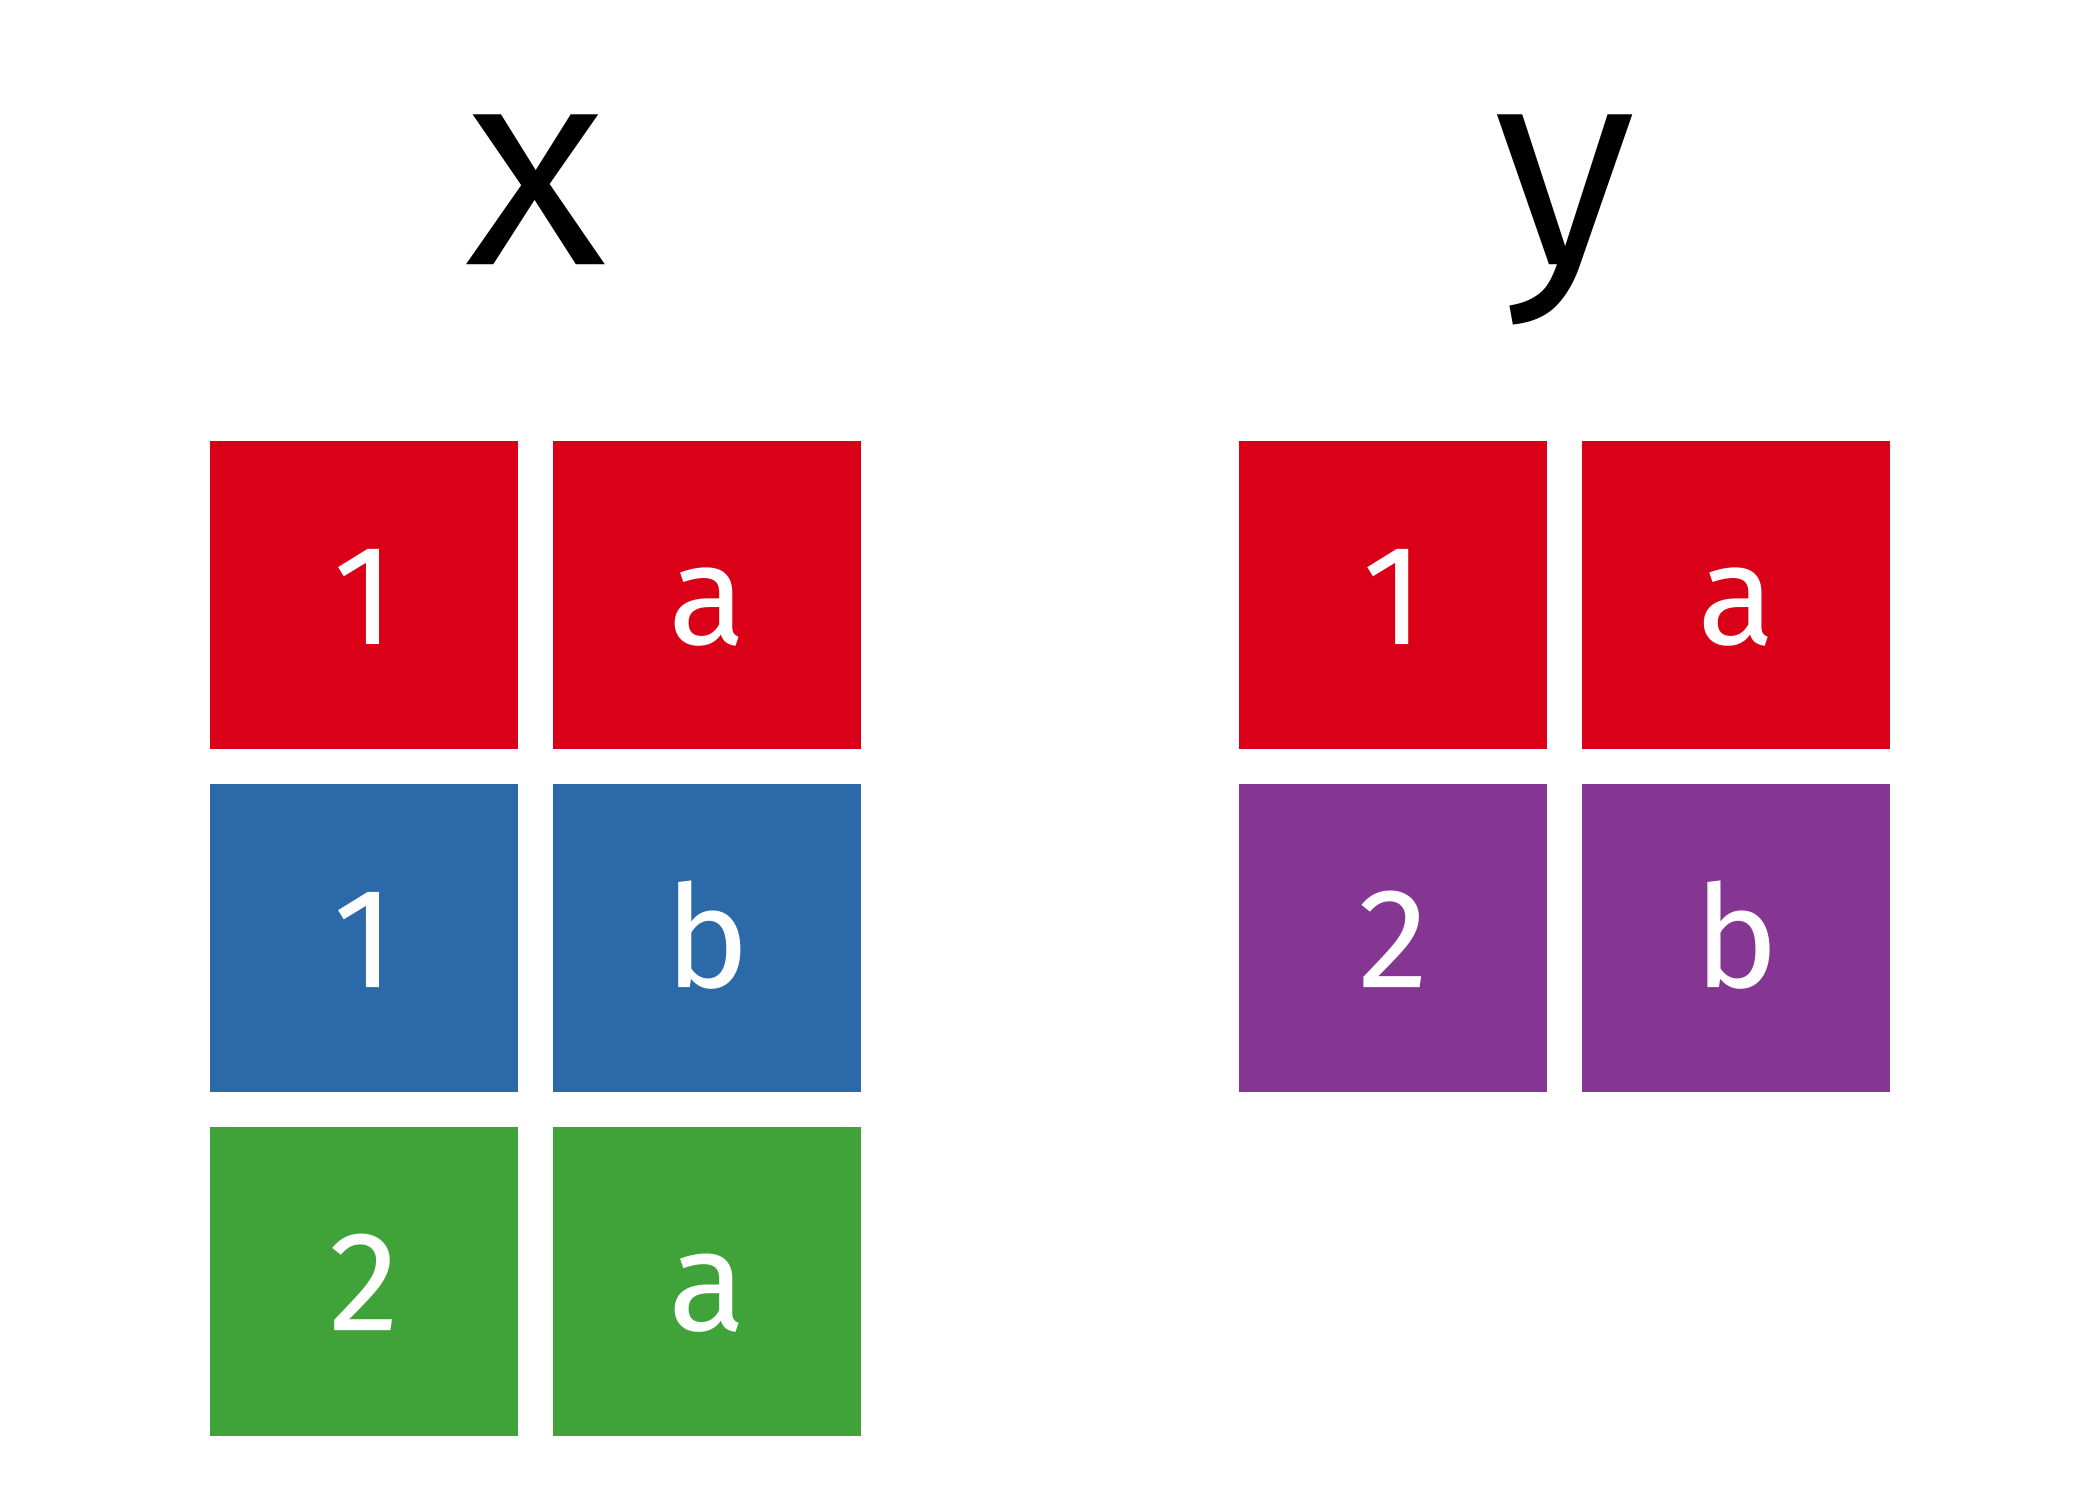
\includegraphics[width=0.5\textwidth,height=\textheight]{original-dfs-set-ops.png}
\caption{\emph{Fonte:
\url{https://www.garrickadenbuie.com/project/tidyexplain/}}}
\end{figure}

\begin{Shaded}
\begin{Highlighting}[]
\CommentTok{#x}
\CommentTok{#> # A tibble: 3 x 2}
\CommentTok{#>   x     y    }
\CommentTok{#>   <chr> <chr>}
\CommentTok{#> 1 1     a    }
\CommentTok{#> 2 1     b    }
\CommentTok{#> 3 2     a}
\CommentTok{#y }
\CommentTok{#> # A tibble: 2 x 2}
\CommentTok{#>   x     y    }
\CommentTok{#>   <chr> <chr>}
\CommentTok{#> 1 1     a    }
\CommentTok{#> 2 2     b}
\end{Highlighting}
\end{Shaded}

\begin{itemize}
\item
  intersect(x, y): retorna apenas observações presentes em x e y
\end{itemize}

\begin{figure}
\centering
\includegraphics[width=0.5\textwidth,height=\textheight]{intersect.gif}
\caption{\emph{Fonte:
\url{https://www.garrickadenbuie.com/project/tidyexplain/}}}
\end{figure}

\begin{Shaded}
\begin{Highlighting}[]
\CommentTok{#intersect(x, y)}
\CommentTok{#> # A tibble: 1 x 2}
\CommentTok{#>   x     y    }
\CommentTok{#>   <chr> <chr>}
\CommentTok{#> 1 1     a}
\end{Highlighting}
\end{Shaded}

\begin{itemize}
\tightlist
\item
  union(x, y): Retorna observações únicas em x e y.
\end{itemize}

\begin{figure}
\centering
\includegraphics[width=0.5\textwidth,height=\textheight]{union.gif}
\caption{\emph{Fonte:
\url{https://www.garrickadenbuie.com/project/tidyexplain/}}}
\end{figure}

\end{document}
